\chapter{Training}


\section{Activation Functions}
\label{sec:activation}
\subsection{Initial \& Convolutional Layers}
At the end of each transition, an elementwise activation function is applied 
following completion of all computations.  For all but the final layer, that 
function is ReLU\footnote{NEEDS CITATION}, defined in figure \ref{fig:relu}.

\begin{figure}[h]
	\centering
	\begin{minipage}{.48\textwidth}
		\begin{equation*}
			relu(x) = \begin{cases}
				0 & x < 0\\
				x & x \geq 0
			\end{cases}
		\end{equation*}
	\end{minipage}
	\begin{minipage}{.48\textwidth}
		\resizebox{\textwidth}{!}{
		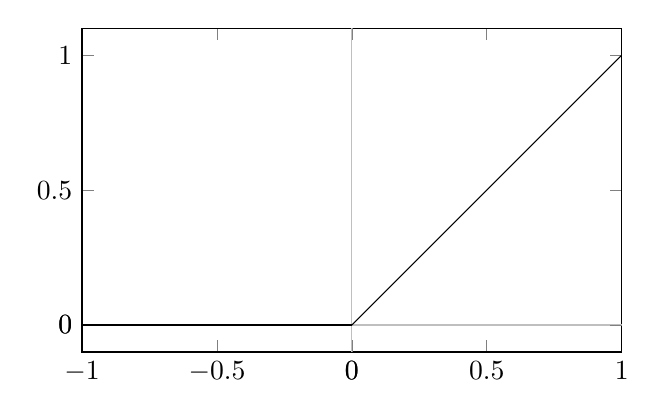
\begin{tikzpicture}
			\begin{axis}[domain=-1:1, unit vector ratio*=1 1 1,
					enlarge x limits=false, extra y ticks=0, extra x ticks=0,
					extra tick style={grid=major}]
				\addplot[color=black][domain=0:1] {x} [mark=none, smooth];
				\addplot[color=black][domain=-1:0] {0} [mark=none smooth];
			\end{axis}
		\end{tikzpicture}
		}
	\end{minipage}
	\caption{ReLU function definition and graph}
	\label{fig:relu}
\end{figure}\noindent

\subsubsection{Alternative Activations}
In addition to ReLU, we considered a sigmoid activation function, as in 
\figref{fig:sigmoid}.

\begin{figure}[h]
	\centering
	\begin{minipage}{.48\textwidth}
		\begin{equation*}
			S(x) = \frac{1}{1 + exp(-x)}
		\end{equation*}
	\end{minipage}
	\begin{minipage}{.35\textwidth}
		\resizebox{\textwidth}{!}{
		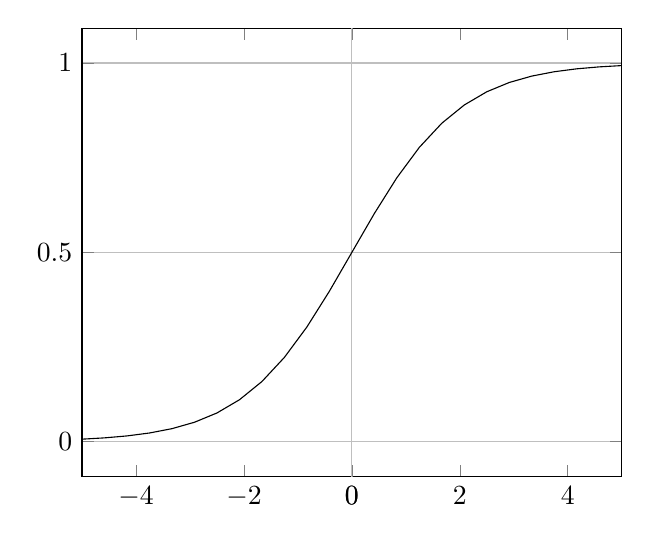
\begin{tikzpicture}
			\begin{axis}[domain=-5:5, ytick={0,.5,1},
					enlarge x limits=false, ymajorgrids, extra x ticks=0,
					extra tick style={grid=major}]
					\addplot[color=black] {1/(1+exp(-x))} [mark=none, smooth];
			\end{axis}
		\end{tikzpicture}
		}
	\end{minipage}
	\caption{Sigmoid function definition and graph}
	\label{fig:sigmoid}
\end{figure}\noindent
However, this function requires that the network have extremely well-tuned 
matrices in order to produce values near zero, and, given our binary generator 
networks, it presents unecessary training difficulty, leading us to use ReLU.


\subsection{Final Layer}
\label{subsec:finalactivation}
Additionally, ReLU's preservation of positive values and elimination of negative 
work in concert with the activation function of the final layer, hyperbolic 
tangent (\figref{fig:tanh}).
The clipping of negative values to 0 in previous layers of the network allows 
greater imprecision in the penultimate layers in order to predict a 0 in the 
output adjacency matrix: rather than needing to fine tune the filters to produce 
exactly 0 for nonexistent connections, the model need only drive the values for 
such neuron pairs into the negatives, and let the application of ReLU correct.  

\begin{wrapfigure}[5]{r}{.45\textwidth}
	\centering
	\vspace{-14pt}
	\resizebox{.43\textwidth}{!}{
		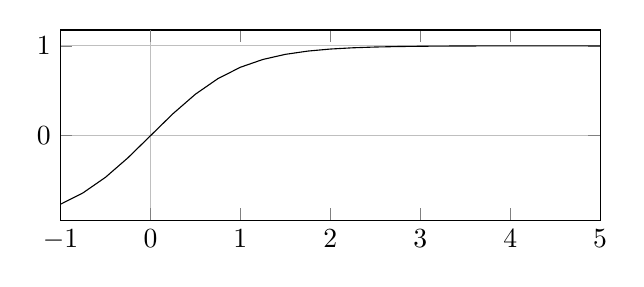
\begin{tikzpicture}
			\begin{axis}[domain=-1:5, unit vector ratio*=1 1 1,
				ytick={0,1}, enlarge x limits=false, ymajorgrids,
				xtick={-1,1,2,3,4,5},
				extra x ticks=0, extra tick style={grid=major}]
				\addplot[color=black] {tanh(x)} [mark=none, smooth];
			\end{axis}
		\end{tikzpicture}
	}
	\caption{Graph of $y=\tanh(x)$}
	\label{fig:tanh}
\end{wrapfigure}
Similarly, the final layer \textit{tanh} allows the network to drive weights for 
probable connections far into the positives, with the activation function 
ultimately truncating them to 1.

\section{Loss \& Optimization}
In a nutshell, backpropagation via gradient descent is a method for training 
neural networks by calculating the extent to which each value in a particular 
layer is responsible for the overall network error on a single data point or 
batch, then correcting that value by an amount commensurate to its error and 
overall learning rate. This process operates from the final layer back to the 
first, hence `backpropagation'.

In order to effectively descend the gradient, a network needs a function 
defining error from the desired output and an algorithm for applying gradient 
descent based on that error and a specified learning rate.

The loss function must provide useful values to the optimizer in order to allow 
effective gradient descent towards the goal, and the optimizer must adjust the 
network fast enough to converge to the target while avoiding converging to a 
suboptimal solution. As the network gets closer to an optimal state, adjusting 
at the same rate as at the start of training will almost invariably overshoot 
the desired configuration. Due to this, the optimizer must dynamically modify 
the extent to which it adjusts the network as training goes on.

\subsection{Loss Function}
% why was this so goddamn hard
\edef\myindent{\the\parindent}
\begin{minipage}{\textwidth}\setlength{\parindent}{\myindent}
\noindent We define a basic custom loss function in order to better fit the 
outputs we expect to see.

For final model output $\mathbb{O}$ and target $\mathbb{T}$, we take the sum 
squared difference, $S$, of the two vectors and the sum over $\mathbb{T}$, 
$S_T$, \eqref{eq:ssd}, and divide these two values to achieve loss 
$L$.\footnotemark
\end{minipage}
\begin{subequations}
	\centering
	\begin{align}
		S &= \sum_i \left(\mathbb{O}_i - \mathbb{T}_i \right)^2
		= \sum_i \left[\left(\mathbb{O} - \mathbb{T})_i \right)\right]^2 &
		S_T &= \sum_i \mathbb{T}_i
		\label{eq:ssd}
	\end{align}
	\begin{equation}
		L = \frac{S}{S_T}
		\label{eq:los}
	\end{equation}
	\label{eq:losscalc}
\end{subequations}

\footnotetext{Recall from \ref{subsubsec:targetdata} that the targets 
$\mathbb{T}$ given to the model are the flattend generator adjacency matrix; 
dimensionality $(1 \times n^2)$.}
Thus, rather than scale loss with the number of total possible connections 
($n^2$) as with a mean squared error, we scale our loss with the number of 
actual connections in the true adjacency matrix, keeping the loss values 
somewhat higher in the early stages of training, yet still falling to levels 
comparable to that of MSE as the model learns to predict appropriately.

%\begin{minipage}{\textwidth}
\subsubsection{Effects}
\label{subsubsec:losseffects}
\begin{wraptable}[5]{r}{.3\textwidth}
	\captionsetup{justification=centering}
	\vspace{-30pt}
	\centering
	\adjacencyT{0 & 0 & 0}{1 & 0 & 0}{1 & 1 & 0}
	\vspace{-5pt}
	\captionof{figure}{\linespread{1.2}\selectfont{}Example adjacency matrix}
	\label{fig:loss_ex}
\end{wraptable}
Consider a model analyzing data from a 3-neuron generator with an adjacency 
matrix as given in \figref{fig:loss_ex}, and suppose that its output is a vector 
containing two correct values and one wrong value.  Then our parameters for 
determining loss by way of \eqref{eq:losscalc} are as follows:
\begin{align*}
	\mathbb{O} &= \begin{bmatrix} 0.0 & 0.0 & 0.0 & 1.0 & 0.0 & 0.0 & 1.0 & 0.0 
			   & 1.0\end{bmatrix}\\
	\mathbb{T} &= \begin{bmatrix} 0.0 & 0.0 & 0.0 & 1.0 & 0.0 & 0.0 & 1.0 & 1.0 
				& 0.0\end{bmatrix}\\
	\left(\mathbb{O} - \mathbb{T}\right)^2 &= \begin{bmatrix} 0.0 & 0.0 & 0.0 & 
		0.0 & 0.0 & 0.0 & 0.0 & 1.0 & 1.0\end{bmatrix}\\
	S 	&= \sum_i \left(\mathbb{O}_i - \mathbb{T}_i \right)^2 = 2.0\\
	S_T &= \sum_i \mathbb{T}_i = 3.0
	\intertext{And our loss is finally determined:}
	L 	&= \frac{S}{S_T} = \frac{2.0}{3.0} = .\overline{6}
\end{align*}
%\end{minipage}
Thus, our loss function `punishes' the network equally for false positives and 
false negatives: due to the squared difference, a 1 where there should be a 0 
adds the same loss as a 0 where there should be a one. This is perhaps not the 
ideal method; see The value produced for each input/target pair is then passed 
to the optimizer.

\subsection{Optimizer Function}
\label{subsec:optimizer}
We used the Adam optimizer\footnote{Citation} as provided by TensorFlow, 
providing different initial learning rates per dataset. Those values were 
arrived at via experimentation. After initializing the optimizer, it is passed 
the loss at each step and performs gradient descent on the trainable matrices.

Adam adjusts its learning rate as time goes on, according to the following 
equation, where $\beta_n^t$ indicates exponentiation by $t$ and $lr$ denotes 
learning rate:
\begin{figure}[h]
	\begin{minipage}[b]{.38\textwidth}
		\centering
		\begin{gather}
			\nonumber
			\beta_1 = 0.9\\
			\nonumber
			\beta_2 = 0.999\\
			\nonumber
			lr_t = lr_{init} \times \frac{\sqrt{1-\beta_2^t}}{1-\beta_1^t}
		\end{gather}
	\end{minipage}
	\hfill
	\begin{minipage}{.6\textwidth}
		\centering
		\resizebox{\textwidth}{!}{
			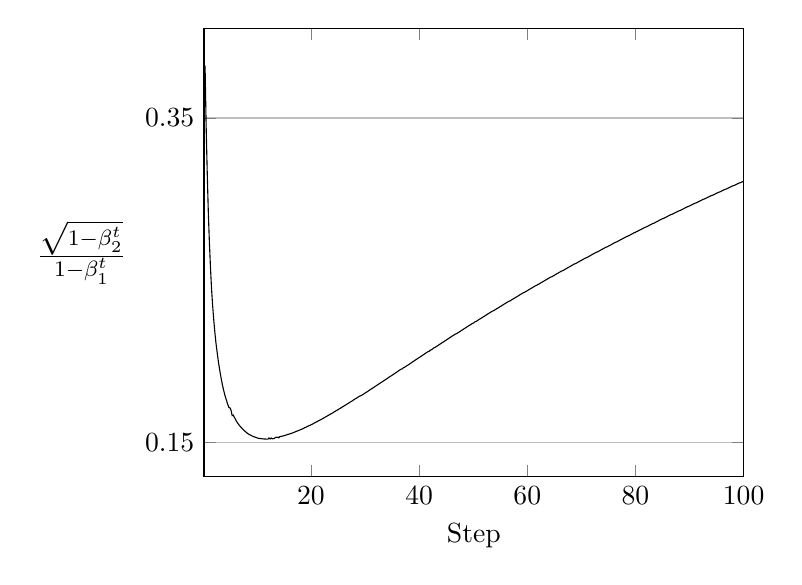
\begin{tikzpicture}
			\begin{axis}[domain=.01:100, ytick={0,.15,.35}, samples=500,
				ylabel=$\frac{\sqrt{1-\beta_2^t}}{1-\beta_1^t}$,
				ylabel style={rotate=-90, font=\large},
					enlarge x limits=false, ymajorgrids, extra x ticks=0,
					extra tick style={grid=major}, xlabel=Step]
					\addplot[color=black] {sqrt(1-.999^x)/(1-.9^x)} [mark=none, 
			smooth];
			\end{axis}
		\end{tikzpicture}
		}
		\captionof{figure}{Adam decay function over 100 steps. Converges 
			asymptotically to 1.}
	\end{minipage}
\end{figure}

\section{Datasets}


\section{Matrix Initialization}
Initially, we seeded our matrices with random values from a normal distribution 
of standard deviation 1.0 and mean 0, using the TensorFlow implementation of 
\texttt{tf.random\_normal(<dimensions>)}. Due, however, to the cumulative nature 
of our matrix operations (in the convolutional layer, for instance, there are 
three separate multiplications \ref{subsubsec:matconvlayer}), we found that the 
values 

\section{Hyperparameter Optimization}
